% Global options
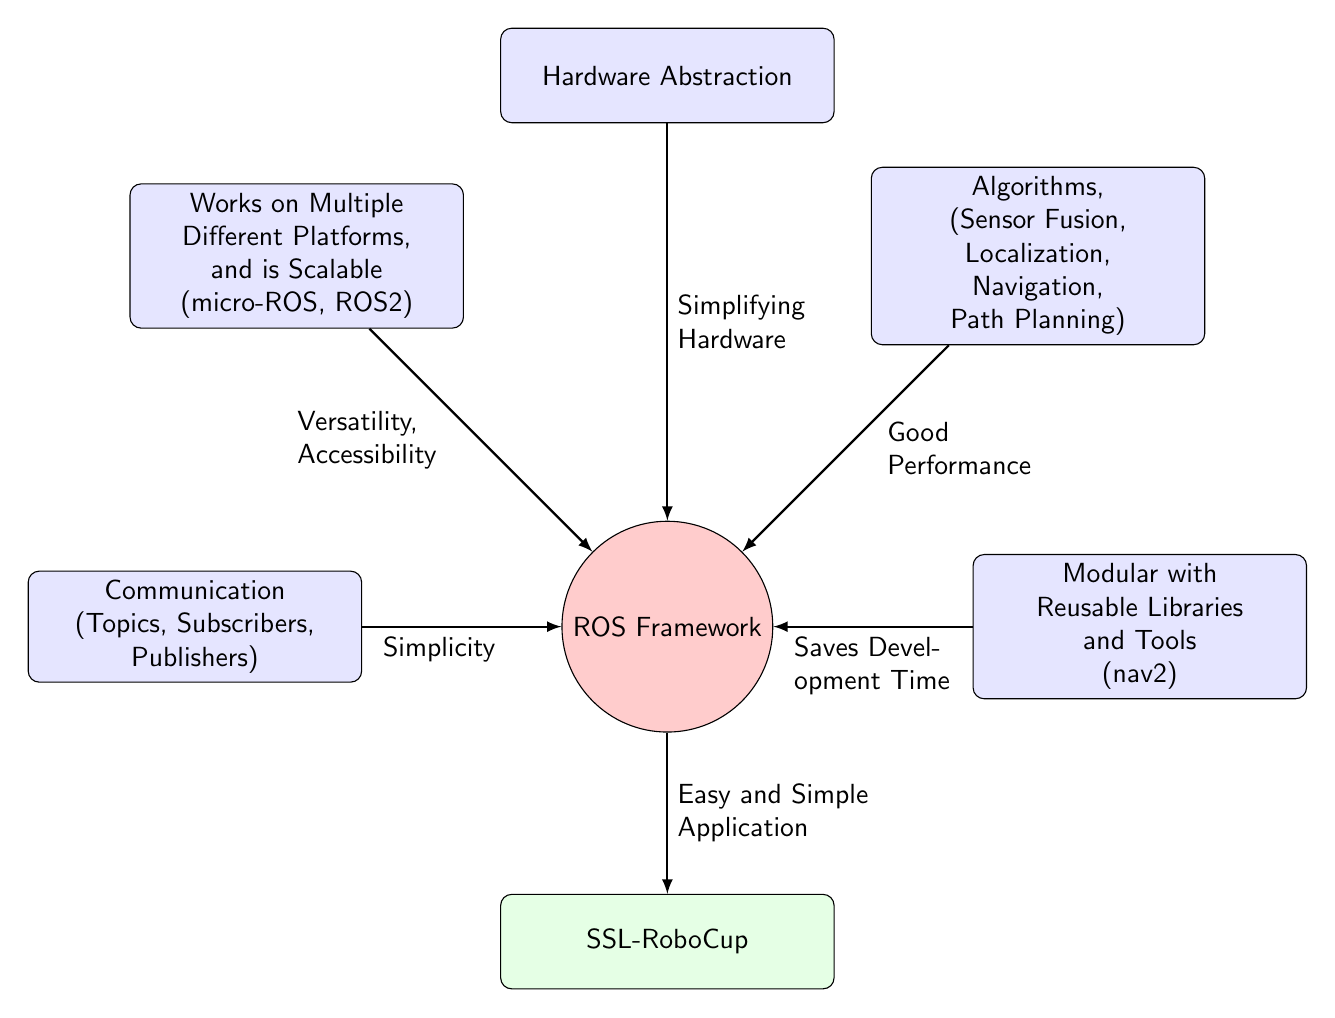
\begin{tikzpicture}[
    font=\sffamily,
    block/.style={rectangle, draw=black, fill=blue!10, text width=4cm, align=center, rounded corners, minimum height=1.2cm},
    arrow/.style={->, thick, >=latex},
    circleblock/.style={circle, draw=black, fill=red!20, minimum size=1.5cm, align=center},
    system/.style={rectangle, draw=black, fill=green!10, text width=2cm, align=center, rounded corners, minimum height=1.2cm},
]
    
    % Core ROS bubble
    \node[circleblock] (ros) {ROS Framework};
    
    % Surrounding blocks
    \node[block, above of=ros, yshift=6cm] (hardware) {Hardware Abstraction};
    \node[block, left of=ros, xshift=-5cm] (communication) {Communication \\ (Topics, Subscribers, \\ Publishers)};
    \node[block, above right of=ros, xshift=4cm, yshift=4cm] (planning) {Algorithms, \\ (Sensor Fusion, \\ Localization, \\ Navigation, \\ Path Planning)};
    \node[block, above left of=ros, xshift=-4cm, yshift=4cm] (crossplatform) {Works on Multiple \\ Different Platforms, \\ and is Scalable \\ (micro-ROS, ROS2)};
    \node[block, right of=ros, xshift=5cm] (reusability) {Modular with \\ Reusable Libraries \\ and Tools \\ (nav2)};
    
    % System-specific example
    \node[system, below of=ros, yshift=-3cm, text width=4cm] (ssl) {SSL-RoboCup};
    
    % Arrows connecting to ROS
    \draw[arrow] (hardware) -- (ros) node[right, midway, text width=3cm] {Simplifying \newline Hardware};
    \draw[arrow] (communication) -- (ros) node[midway, below, text width=2cm] {Simplicity};
    \draw[arrow] (planning) -- (ros) node[midway, below, right, xshift=0.4cm, text width=3cm] {Good \newline Performance};
    \draw[arrow] (crossplatform) -- (ros) node[midway, below, left, xshift=0.8cm, text width=3cm] {Versatility, \newline Accessibility};
    \draw[arrow] (reusability) -- (ros) node[midway, below, text width=2cm] {Saves Development Time};
    
    % Connection to the system
    \draw[arrow] (ros) -- (ssl) node[midway, right, text width=3cm] {Easy and Simple \newline Application};
    
\end{tikzpicture}